\documentclass[deutsch]{lib/llncs/llncs}
\usepackage{lib/llncs/llncsdoc}
\usepackage[ngerman]{babel}
\usepackage[utf8]{inputenc}
\usepackage{hyperref}
\usepackage{graphicx}
\usepackage{lib/picins/picins}
\usepackage[nottoc]{tocbibind}


\begin{document}
\markboth
{Anwendung des ''Technology Acceptance Model'' zur Akzeptanzbestimmung qualifizierter elektronischer  Fernsignaturen im Unternehmensumfeld}
{Anwendung des ''Technology Acceptance Model'' zur Akzeptanzbestimmung qualifizierter elektronischer  Fernsignaturen im Unternehmensumfeld}
\thispagestyle{empty}


\begin{flushleft}
\LARGE\bfseries Anwendung des ''Technology Acceptance Model'' zur Akzeptanzbestimmung qualifizierter elektronischer  Fernsignaturen im Unternehmensumfeld


\end{flushleft}
\rule{\textwidth}{1pt}
\vspace{2pt}


\begin{flushright}
\Huge


\begin{tabular}{@{}l}
Interdisziplinäre und \\
sozialwissenschaftliche \\
Reflexion der Informatik 2\\\\
Wintersemester 2017/2018\\\\
Frank Dreyer\\
Matrikelnummer: 741827\\\\
07.02.2018\\[6pt]
\end{tabular}


\end{flushright}
\rule{\textwidth}{1pt}
\vfill

\newpage
\tableofcontents
\newpage\vspace{2pt}


\section{Grundlagen}


\subsection{Technology Acceptance Model}
Das \textit{Technology Acceptance Model} \cite{Zitat01}, kurz TAM, ist ein von Davis entwickeltes Akzeptanzmodell, welches versucht, auf Grundlage des von Ajzen und Fishbein entwickelten sozialpsychologischem Modells \textit{Theory of Reasond Action} (TRA) \cite{Zitat04}, Aussagen darüber treffen zu können warum eine Technologie von einer Person akzeptiert wird oder nicht. Dabei wird angenommen, dass eine Person mit positiver Nutzungseinstellung zur Technologie, diese auch tatsächlich verwendet. (Vgl. \cite[p. 237]{Zitat03}) Diese Nutzungseinstellung hängt wiederum maßgeblich von den Faktoren 'wahrgenommener Nutzen' und 'wahrgenommener Bedienungskomfort' ab. \\
Der 'wahrgenommene Nutzen' beschreibt das subjektiv Empfinden, dass sich eine Technologie positiv auf die Steigerung der eigenen Arbeitsleistung in einem organisatorischem Kontext auswirkt.  (Vgl. \cite[p. 320]{Zitat02}) \\
Der 'wahrgenommene Bedienungskomfort' bezeichnet das subjektive Empfinden, dass die Verwendung einer Technologie mit wenig Aufwand verbunden ist, bzw. einfach zu benutzen ist. (Vgl. \cite[p. 320]{Zitat02}) \\
Bandow und Holzmüller fassen die Auswirkung dieser beiden Determinanten folgendermaßen zusammen: ''Je größer der Nutzen eines Informationssystems und je einfacher dessen Bedienbarkeit, desto eher ist der Anwender dazu bereit, das neue System zu nutzen.'' (Vgl. \cite[p. 237]{Zitat03}) \\
Auf diese beiden Einflussfaktoren wirken wiederum 'externe Variablen', die unter anderem demografische und persönliche Merkmale des Akteurs umfassen, im Originalmodell allerdings nicht weiter spezifiziert werden. (Vgl. \cite[p. 21]{Zitat01}) \\
Abbildung 1 illustriert das Modell.
\begin{figure}
	\centering
	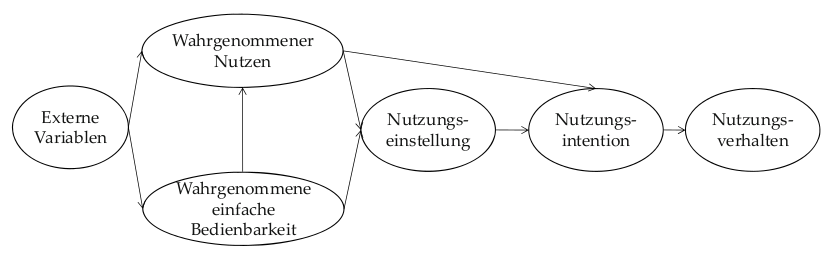
\includegraphics[scale=0.40]{img/abbildung1.png}
	\caption{\textit{Technology Acceptance Model} (Vgl. \cite[p. 237]{Zitat03})}
\end{figure}


\bibliographystyle{amsalpha}
\bibliography{lit/lit}


\end{document}
